\section{Befehlssatzarchitektur}
\label{sec:befehlssatzarchitektur}

\begin{figure}[ht]
  \centering
  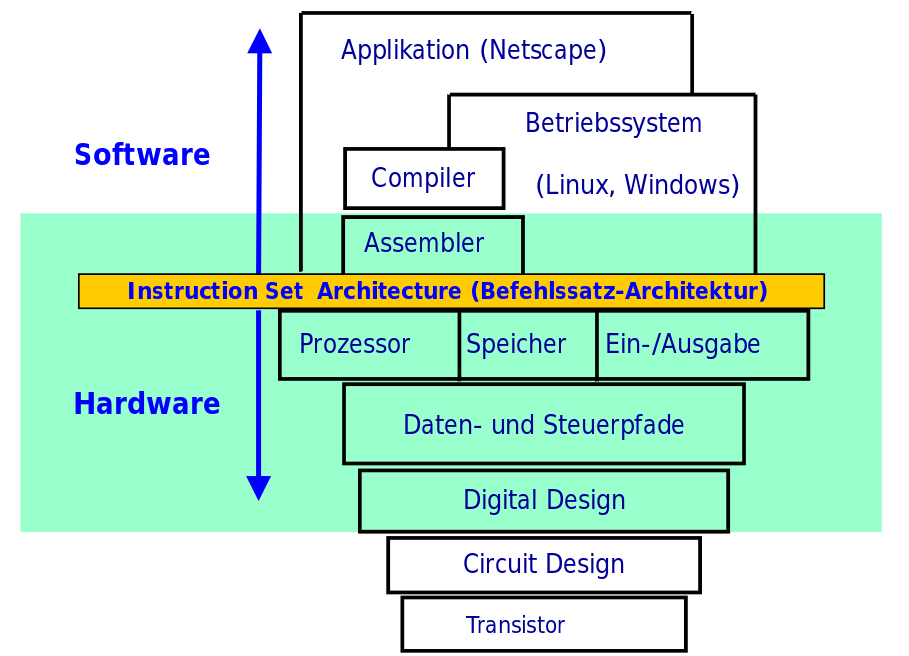
\includegraphics[width=0.33\textwidth]{ISA}
  \label{ISA}
\end{figure}

\textbf{ISA -- Aufgaben}
\begin{items}
	\item Wie werden Daten repräsentiert?
	\item Wo werden Daten gespeichert?
	\item Welche Operationen können auf den Daten ausgeführt werden?
	\item Wie werden die Befehle codiert?
	\item Wie wird auf die Daten zugegriffen?
	\item $\leadsto$ abstrahiert Hardware für den Maschinenprogrammierer
\end{items}

\textbf{Ausführungsmodelle}
\begin{figure}[ht]
  \centering
  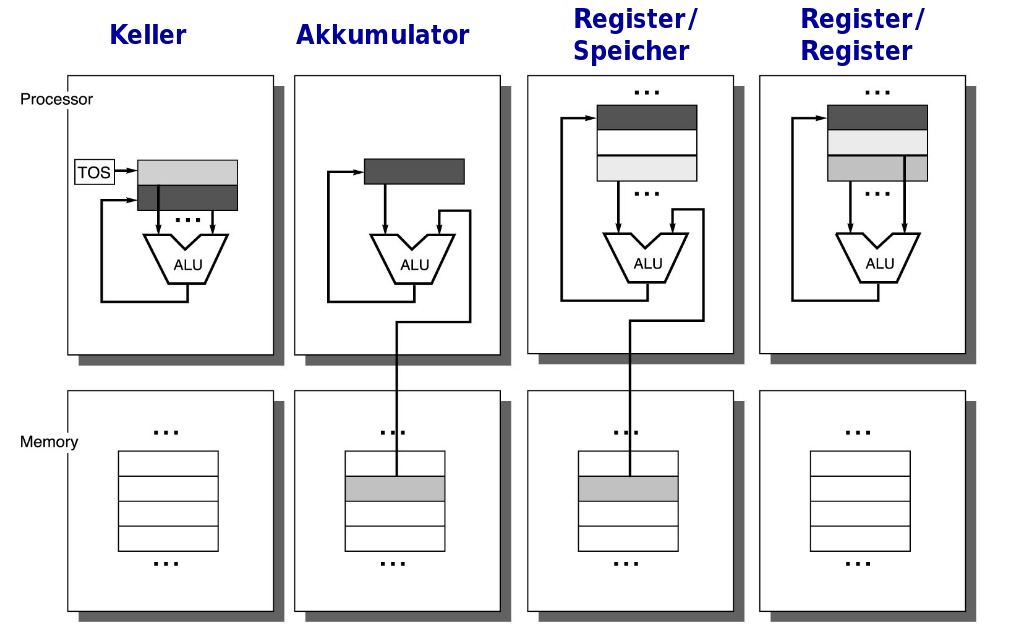
\includegraphics[width=0.33\textwidth]{Ausfuehrungsmodelle}
  \label{Ausfuehrungsmodelle}
\end{figure}

\textbf{Ausführungsmodell -- Register-Register}
\begin{items}
	\item Alle Operanden und Ergebnis stehen in Allzweckregistern
	\item \underline{Load/Store}: Bestimmte Befehle holen Operanden aus Hauptspeicher, schreiben Inhalte von Registern in Speicher
	\item \underline{Dreiadressformat}
	\begin{align*}
		\text{\code{load R2,A}} &\quad \text{\code{R2<-mem[A]}} \\
		\text{\code{load R3,B}} &\quad \text{\code{R3<-mem[B]}} \\
		\text{\code{add R1,R2,R3}} &\quad \text{\code{R1<-R2+R3}} \\
		\text{\code{store C,R1}} &\quad \text{\code{mem[C]<-R1}}
	\end{align*}
	\item \underline{Vorteile}: Einfaches und festes Befehlsformat, einfaches Code-Generierungsmodell, etwa gleiche Ausführungszeit der Befehle
	\item \underline{Nachteile}: Höhere Anzahl von Befehlen im Vergleich zu Architekturen mit Speicherreferenzen, längere Programme
\end{items}

\textbf{Ausführungsmodell -- Register-Speicher}
\begin{items}
	\item Ein Operand im Speicher, ein Operand im Register, Ergebnis in Speicher oder Register
	\item Explizite Adressierung mit/ohne Überdeckung
	\item \underline{Zweiadressformat}
	\begin{align*}
		\text{\code{add A,R1}} &\quad \text{\code{mem[A]<-mem[A]+R1}} \\
		\text{\code{add R1,A}} &\quad \text{\code{R1<-R1+mem[A]}}
	\end{align*}
	\item \underline{Vorteile}: Zugriff auf Daten ohne vorherige Ladeoperationen, Befehlsformat-Kodierung $\leadsto$ höhere Code-Dichte
	\item \underline{Nachteile}: Keine gleiche Operanden-Behandlung bei Überdeckungen, Taktzyklen pro Instruktion von Adressrechnung abhängig
\end{items}

\newpage

\textbf{Ausführungsmodell -- Akkumulator-Register}
\begin{items}
	\item \underline{Akkumulator}: Ausgezeichnetes Register, dient als Quelle eines Operanden und als Ziel für das Resultat (zweistellige Operationen)
	\item Implizite und überdeckte Adressierung
	\item Spezielle Befehle ermöglichen Operanden-Transport
	\item \underline{Einadressformat}
	\begin{align*}
		\text{\code{add A}} &\quad \text{\code{acc<-acc+mem[A]}} \\
		\text{\code{addx A}} &\quad \text{\code{acc<-acc+mem[A+x]}} \\
		\text{\code{add R1}} &\quad \text{\code{acc<-acc+R1}}
	\end{align*}
\end{items}

\textbf{Ausführungsmodell -- Keller}
\begin{items}
	\item Operanden einer zweistelligen Operation stehen auf den obersten zwei Kellerelementen
	\item Ergebnis wird auf Keller abgelegt
	\item Implizite Adressierung über Kellerzeiger (\code{tos})
	\item Überdeckung
	\item \underline{Nulladressformat}
	\begin{align*}
		\text{\code{add}} &\quad \text{\code{tos<-tos+next}}
	\end{align*}
\end{items}

\textbf{Ausführungsmodelle -- Übersicht} \\
\begin{items}
	\item 
	\begin{center}
		\code{C=A+B; D=C-B}
	\end{center}
	\begin{figure}[ht]
	  \centering
	  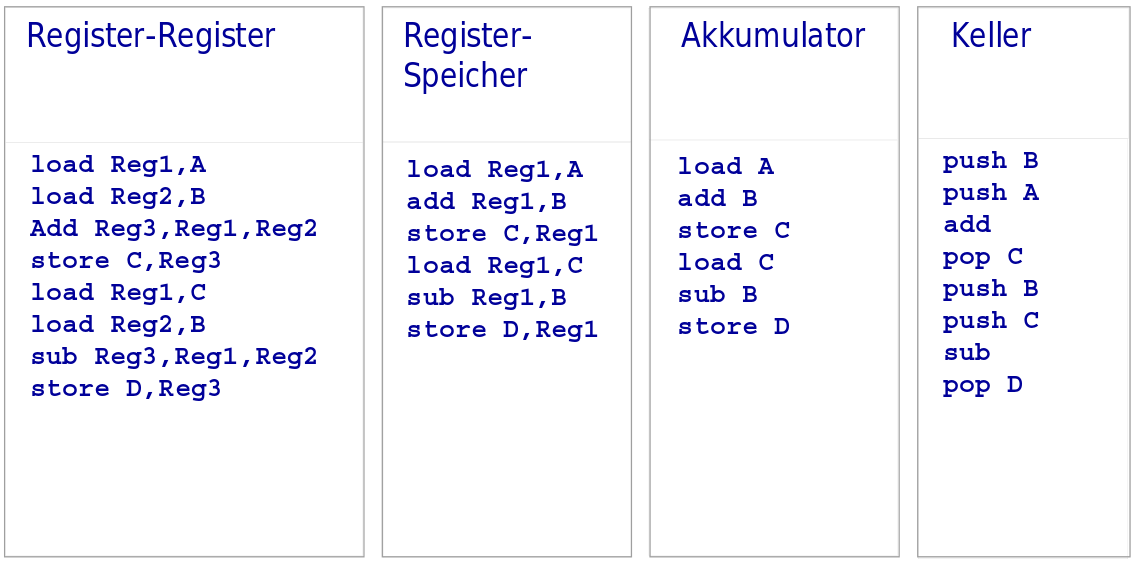
\includegraphics[width=0.33\textwidth]{UebersichtISA}
	  \label{UebersichtISA}
	\end{figure}
\end{items}

\textbf{Architektur -- Datentypen}
\begin{items}
	\item = Datenformat + inhaltliche Interpretation
	\item Alternative: Datentyparchitektur (Daten führen Typinformation mit sich)
	\item Datentyp nicht von Hardware unterstützt $\leadsto$ Programm muss Datentyp auf elementare Datentypen zurückführen
	\item \underline{Standardformate}:
	\begin{enumeration}
		\item Byte: 8 Bit
		\item Halbwort: 16 Bit
		\item Wort: 32 Bit
		\item Doppelwort: 64 Bit
	\end{enumeration}
	\item \underline{Vorzeichenlose Dualzahl}:
	\begin{figure}[ht]
	  \centering
	  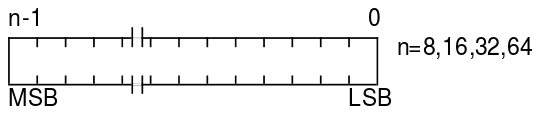
\includegraphics[width=0.33\textwidth]{DualzahlVorzeichenlos}
	  \label{DualzahlVorzeichenlos}
	\end{figure}
	\item \underline{2er-Komplement} (signed Integer):
	\begin{figure}[ht]
	  \centering
	  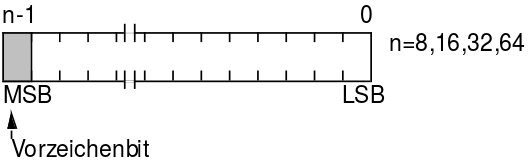
\includegraphics[width=0.33\textwidth]{ZweierKomplement}
	  \label{ZweierKomplement}
	\end{figure}
	\newpage
	\item \underline{BCD (gepackt)}: ein Halbbyte codiert eine Zahl
	\begin{figure}[ht]
	  \centering
	  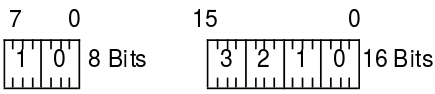
\includegraphics[width=0.33\textwidth]{BCDPacked}
	  \label{BCDPacked}
	\end{figure}
	\item \underline{BCD (ungepackt)}: ein Byte codiert eine Zahl
	\begin{figure}[ht]
	  \centering
	  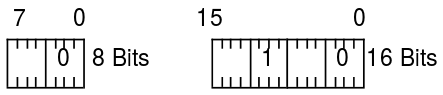
\includegraphics[width=0.33\textwidth]{BCDUnpacked}
	  \label{BCDUnpacked}
	\end{figure}
	\item \underline{Gleitkommazahlen}: Siehe IEEE-Standard oben
	\item \underline{Bitfeld}: Darstellung/Verarbeitung von Bitvektoren, vorzeichenlosen Dualzahlen, Zweierkomplementzahlen - Darstellung durch Byte-Adresse und Bitfeld-Offset
	\begin{figure}[ht]
	  \centering
	  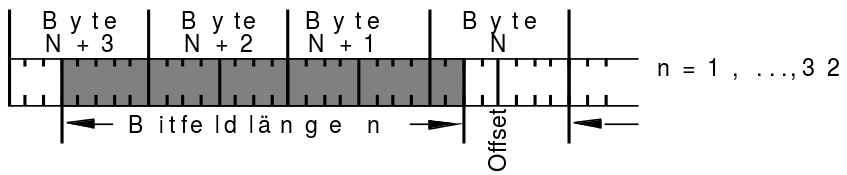
\includegraphics[width=0.33\textwidth]{Bitfeld}
	  \label{Bitfeld}
	\end{figure}
	\item \underline{String}: Aufeinanderfolgend gespeicherte Bytes, enthalten meist ASCII-Zeichen
\end{items}

\textbf{Speicheradressierung -- Datenzugriff}
\begin{enumeration}
	\item \underline{Byte-adressierbarer Speicher}: Jedes Byte ist über eine bestimmte Adresse adressierbar
	\item \underline{Wort-organisierter Speicher}: Zugriffsbreite = Datenbusbreite (32/64/... Bit)
\end{enumeration}

\textbf{Speicheradressierung -- Alignment}
\begin{items}
	\item \underline{Data Alignment}: Datum ($s$ Bytes) ist ausgerichtet abgelegt $\Leftrightarrow$ seine Adresse $A$ ist derart, dass $A \text{ mod } s = 0$
	\item \underline{Data Misalignment}: Daten an beliebiegen Adressen gespeichert
	\begin{items}
		\item \textbf{Vorteile}: Lückenlose Speichernutzung
		\item \textbf{Nachteile}: zusätzliche Speicherzugriffe nötig
	\end{items}
	\item \underline{Little Endian}: Niedrigstwertigstes Byte an der niedrigsten Adresse
	\item \underline{Big Endian}: Niegrigstwertigstes Byte an der höchsten Adresse
\end{items}

\textbf{Speicheradressierung -- Adressierungsarten}
\begin{enumeration}
	\item \underline{Programmadresse}: Im Programm vorliegende Adressen (Prozessor erzeugt aus Programmadressen Prozessadressen mittels Indexmodifikation/Substitution/relativer Adressierung/offener Basisadressierung)
	\item \underline{Prozessadresse} (effektive Adresse): Vom Prozessor verwendet (Prozessor erzeugt nach OS-Angaben aus Prozessadressen Maschinenadressen mittels verdeckter Basisadressierung/Seitenadressierung) - Grund: beliebige Lage des Programms und seiner Werte, partielle Lagerung im Speicher 
	\item \underline{Maschinenadresse}: Vom Prozessor gegenüber Hauptspeicher verwendet
\end{enumeration}

\textbf{Instruction Set}
\begin{items}
	\item legt Grundoperationen eines Prozessors fest
	\item Befehlsarten:
	\begin{enumeration}
		\item Transport
		\item Arithmetik/Logik
		\item Schieben/Rotieren
		\item Multimedia
		\item Gleitkomma
		\item Programmsteuerung
		\item Systemsteuerung
		\item Synchronisation
	\end{enumeration}
\end{items}

\textbf{Instruction Set -- Formate}
\begin{items}
	\item \underline{Befehlsformat} legt Befehlscodierung fest
	\item \underline{Befehlscodierung}: \code{[opcode] [parameter1] ...}
	\item \underline{Adressformate}: vier Befehlssatzklassen:
	\begin{enumeration}
		\item Dreiadressformat: \code{[opcode] [dest] [src1] [src2]}
		\item Zweiadressformat: \code{[opcode] [dest/src1] [src2]}
		\item Einadressformat: \code{[opcode] [src]}
		\item Nulladressformat: \code{[opcode]}
	\end{enumeration}
\end{items}

\textbf{Instruction Set -- MIPS-Prozessor}
\begin{items}
	\item Alle Befehle 32 Bit lang
	\item \underline{Befehlstypen}: 
	\begin{enumeration}
		\item \textbf{Typ R}: Register-Register-Befehle
			\begin{figure}[ht]
			  \centering
			  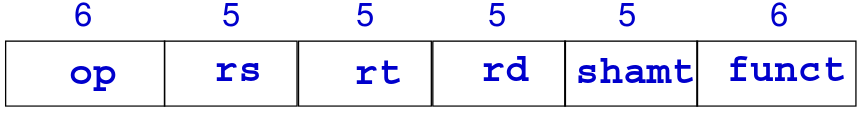
\includegraphics[width=0.33\textwidth]{MIPS-R}
			  \label{MIPS-R}
			\end{figure}
		\item \textbf{Typ I}: Lade-/Speicher-Befehle
			\begin{figure}[ht]
			  \centering
			  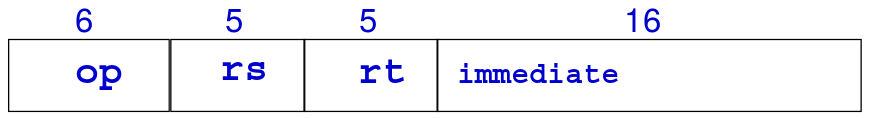
\includegraphics[width=0.33\textwidth]{MIPS-I}
			  \label{MIPS-I}
			\end{figure}
		\item \textbf{Typ J}: Sprungbefehle
			\begin{figure}[ht]
			  \centering
			  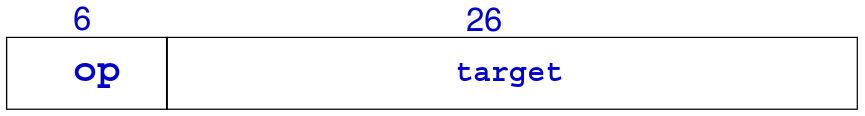
\includegraphics[width=0.33\textwidth]{MIPS-J}
			  \label{MIPS-J}
			\end{figure}
	\end{enumeration}
	\item Abkürzungen: \\*
	\begin{tabular}{ l l }
		\code{I} & Immediate (direkt) \\
		\code{J} & Jump (Sprung) \\
		\code{R} & Register \\
		\code{op} & 6 Bit, Opcode des Befehls \\
		\code{rs} & 5 Bit, Kodierung eines Quellenregisters/Zielregisters \\
		\code{immediate} & 16 Bit, unmittelbarer Wert/Adressverschiebung \\
		\code{target} & 26 Bit, Sprungadresse \\
		\code{rd} & 5 Bit, Kodierung des Zielregisters \\
		\code{shamt} & 5 Bit, Größe einer Verschiebung (shift amount) \\
		\code{funct} & 6 Bit, Codierung der Funktion (function)
	\end{tabular}
\end{items}

\textbf{Adressierung -- Berechnung}
\begin{items}
	\item \underline{Adressierungsarten}: Verschiedene Möglichkeiten, die Adresse eines Operanden/Sprungziels zu berechnen
	\item \underline{Früher}: Adressen in Befehlen absolut vorgegeben $\leadsto$ Programme lageabhängig
	\item \underline{Heute}: \emph{dynamische Adressberechnung}: \\*
		Programmadresse $\leadsto$ logische Adresse $\leadsto$ physikalische Adresse
\end{items}

\textbf{Adressierungsarten}
\begin{enumeration}
	\item \underline{Register-Adressierung}
	\begin{enumeration}
		\item implizit: Flag
		\item explizit
	\end{enumeration}
	\item \underline{einstufige Speicher-Adressierung}
	\begin{enumeration}
		\item unmittelbar
		\item direkt: absolut, Zero-Page, Seiten(-Register)
		\item Register-indirekt
		\item indiziert: Speicher-relativ, Register-relativ, Register-relativ mit Index
		\item Programmzähler-relativ
	\end{enumeration}
	\item \underline{zweistufige Speicher-Adressierung}
	\begin{enumeration}
		\item indirekt absolut
		\item indirekt Register-absolut
		\item indirekt indiziert: Speicher-relativ, Register-relativ, Register-relativ mit Index
		\item indiziert indirekt
		\item indirekt Programmzähler-relativ
	\end{enumeration}
\end{enumeration}

\newpage

\textbf{Adressierungsarten -- Register-Adressierung}
\begin{items}
	\item Operanad steht bereits im Register $\leadsto$ kein Speicherzugriff nötig
	\item \underline{Implizite Adressierung}: Nummer des Registers ist im Opcode-Feld codiert enthalten \\* \textbf{Beispiel}: \code{LSRA} (Verschiebe Akkumulatorinhalt eine Bitposition nach rechts)
		\begin{figure}[ht]
		  \centering
		  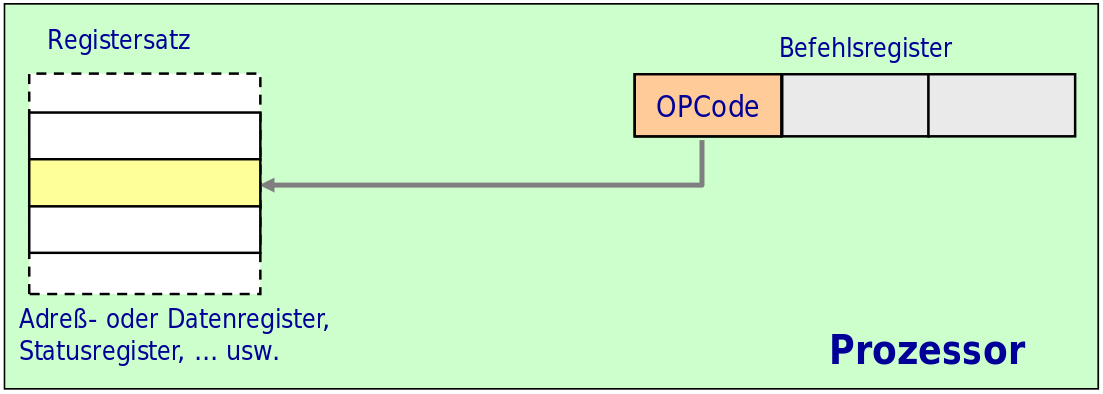
\includegraphics[width=0.33\textwidth]{ImpliziteRegisterAdressierung}
		  \label{ImpliziteRegisterAdressierung}
		\end{figure}
	\item \underline{Flag-Adressierung}: Spezialfall der impliziten Adressierung: Nur ein Bit (=Flag) wird im Register angesprochen \\* \textbf{Beispiel}: \code{SEI/CLI} (set/clear interrupt flag)
		\begin{figure}[ht]
		  \centering
		  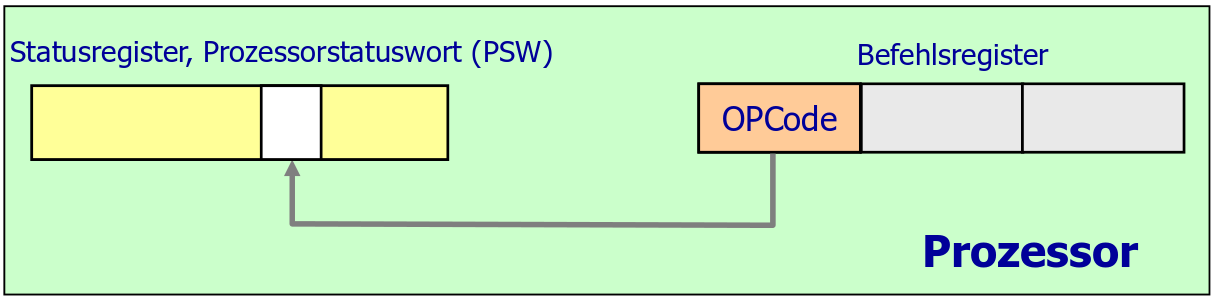
\includegraphics[width=0.33\textwidth]{FlagAdressierung}
		  \label{FlagAdressierung}
		\end{figure}
	\item \underline{Explizite Adressierung}: Registermnummer wird im Operandenfeld angegeben \\* \textbf{Beispiel}: \code{DEC R0} (Dekrementiere Register R0)
		\begin{figure}[ht]
		  \centering
		  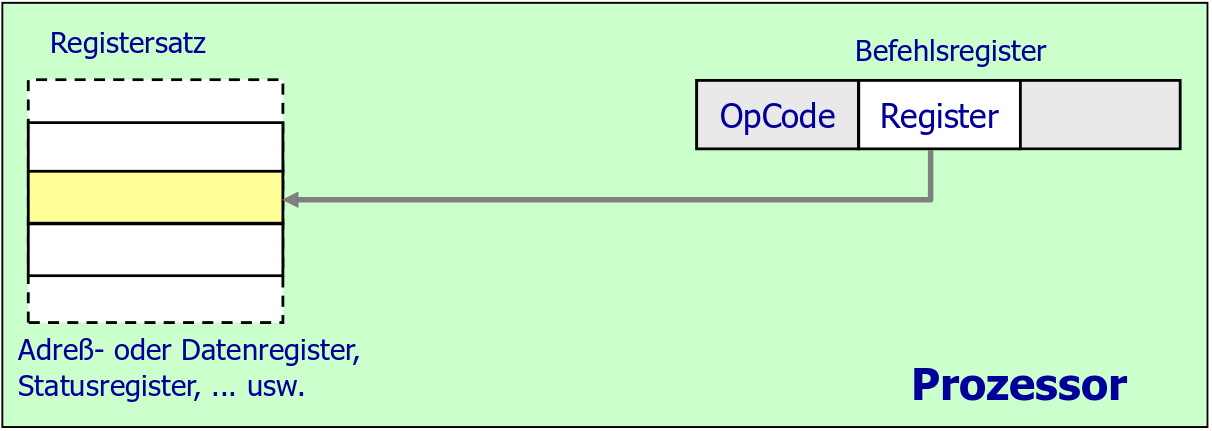
\includegraphics[width=0.33\textwidth]{ExpliziteRegisterAdressierung}
		  \label{ExpliziteRegisterAdressierung}
		\end{figure}
\end{items}

\textbf{Adressierungsarten -- Einstufige Speicher-Adressierung}
\begin{items}
	\item Eine Adressberechnung ist zur Ermittlung der effektiven Adresse nötig $\leadsto$ keine mehrfachen Speicherzugriffe zur Adressermittlung
	\item \underline{Unmittelbare Adressierung}: Befehl enthält nicht Adresse des Operanden, sondern Operand selbst (Opcode und Operand stehen hintereinander im Speicher) \\* \textbf{Beispiel}: \code{LDA #\$A3} (Lade Akkumulator mit Sedezimalwert \code{\$A3})
		\begin{figure}[H]
		  \centering
		  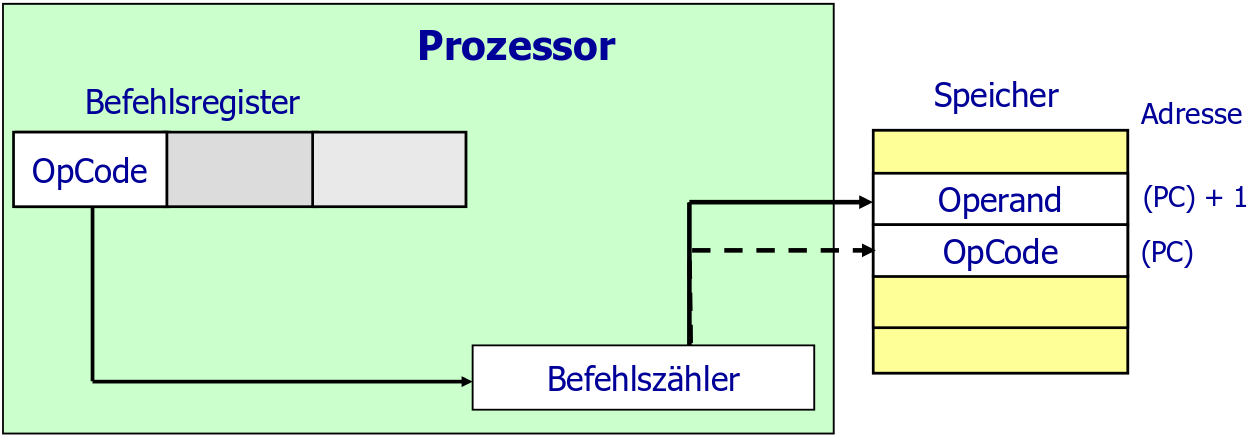
\includegraphics[width=0.33\textwidth]{UnmittelbareAdressierung}
		  \label{UnmittelbareAdressierung}
		\end{figure}
	\item \underline{Direkte Adressierung}: Befehl enthält nach Opcode logische Adresse des Operanden, aber keine Vorschriften zur Manipulation
	\begin{enumerate}
		\item \textbf{Absolute Adressierung}: Speicherwort enthält vollständige (absolute) Operandenadresse \\* Beispiel: \code{JMP \$07FE} (Springe zur Adresse \code{\$07FE})
		\begin{figure}[H]
		  \centering
		  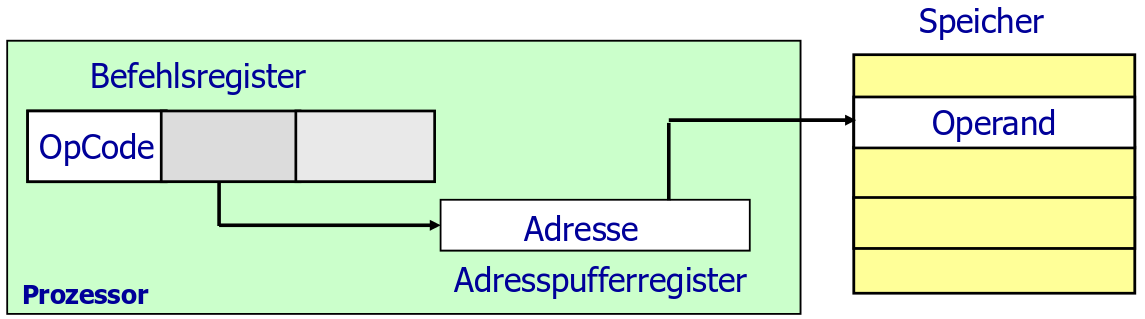
\includegraphics[width=0.33\textwidth]{AbsoluteAdressierung}
		  \label{AbsoluteAdressierung}
		\end{figure}
		\item \textbf{Seitenadressierung}: Im Befehl nur Kurz-Adresse (niederwertige Teil der Adresse). \\* Zero-Page: Höherwertiger Teil: \code{0}-Bits \\* Seiten-Register: Höherwertiger Adressteil wird in Prozessorregister bereitgestellt
	\end{enumerate}

	\item \underline{Register-indirekte Adressierung}: Im Opcode angegebenes Adressregister enthält Adresse des Operanten (=\emph{Pointer}) \\* \textbf{Beispiel}: \code{LD R1, (A0)} (Lade Register \code{R1} mit Inhalt des in \code{A0} angegebenen Speicherwortes)
	\begin{items}
		\item Im Register stehende Adresse oft Anfang/Ende eines Tabellenbereiches, deswegen Hilfsmethoden:
		\item \textbf{Postinkrement}: Nach Befehlsausführung Registerinhalt inkrementieren und auf nächste Speicherzelle zeigen (z.B. \code{INC (R0)+}: Inkrementiere Speicherwortinhalt, das von \code{R0} adressiert wird, danach Inhalt von \code{R0})
		\item \textbf{Predekrement}: Vor Befehlsausführung Registerinhalt erniedrigen und auf vorhergehende Speicherzelle zeigen (z.B. \code{CLR -(R0)}: Dekrementiere Inhalt von \code{R0}, lösche dann durch \code{R0} adressiertes Speicherwort)
	\end{items}
		\begin{figure}[ht]
		  \centering
		  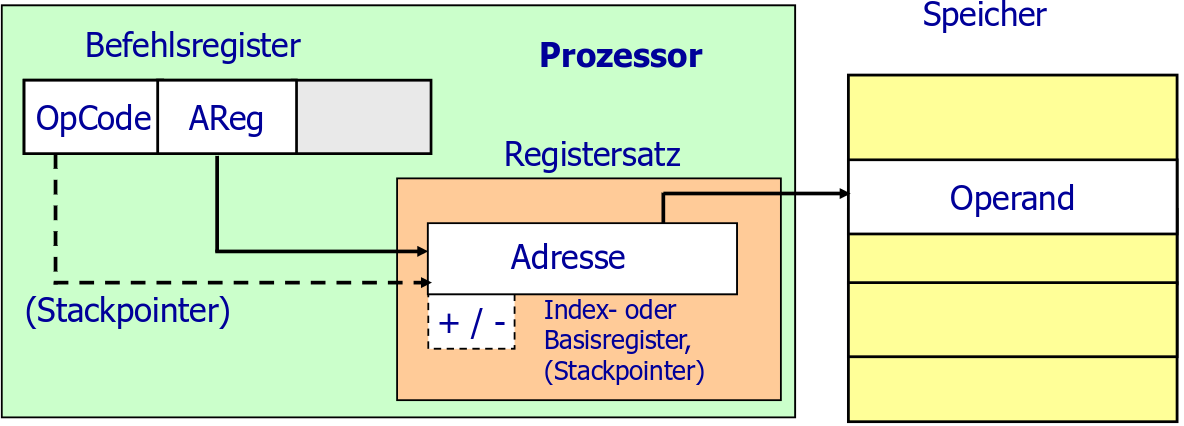
\includegraphics[width=0.33\textwidth]{RegisterIndirekteAdressierung}
		  \label{RegisterIndirekteAdressierung}
		\end{figure}

	\item \underline{Indizierte Adressierung}: Effektive Adresse wird durch Addition eines Registerinhalts zu angegebenem Basiswert berechnet
	\begin{enumeration}
		\item \textbf{Speicher-relative Adressierung}: Basiswert wird als absolute Adresse im Befehl vorgegeben \\* Beispiel: \code{ST R1,\$A704 (R0)} (Speichere Inhalt von \code{R1} in Speicherwort, dessen Adresse man durch Addition des Inhalts von \code{R0} zu Basis \code{\$A704} erhält)
		\begin{figure}[H]
		  \centering
		  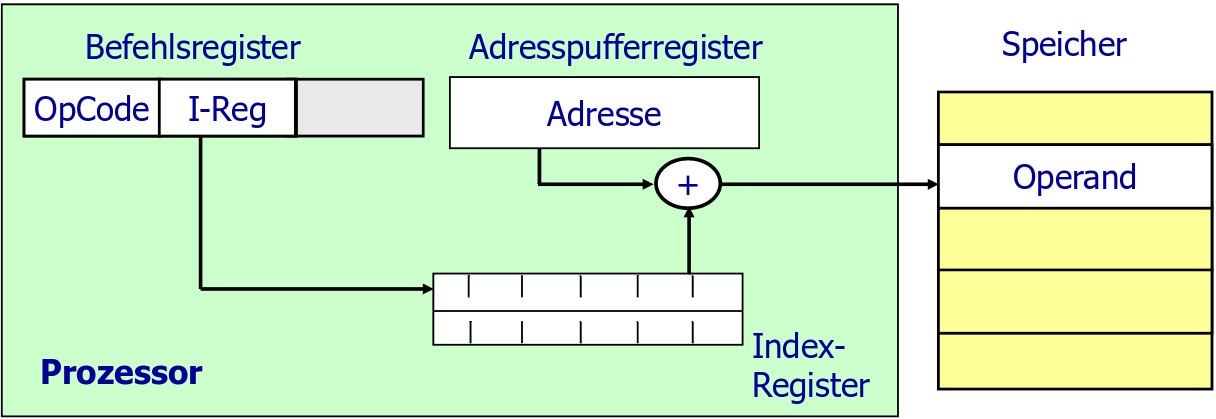
\includegraphics[width=0.33\textwidth]{SpeicherRelativeAdressierung}
		  \label{SpeicherRelativeAdressierung}
		\end{figure}
		\item \textbf{Register-relative Adressierung}: Basiswert befindet sich in Basisregister, verwiesen im \code{BReg}-Feld des Opcodes \\* Beispiel: \code{CLR \$A7 (B0)} (Lösche Speicherwort, dass man durch Addition von \code{\$A7} zu \code{B0} erhält)
		\begin{figure}[H]
		  \centering
		  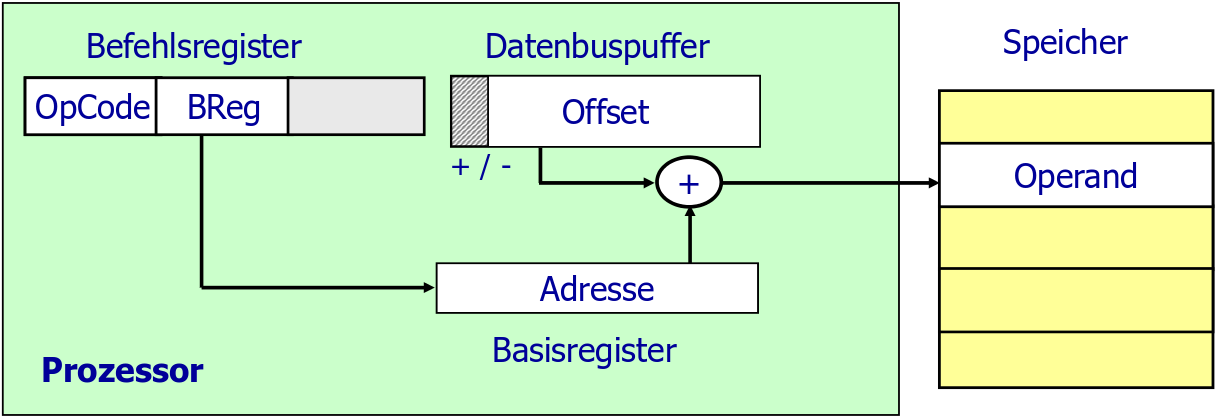
\includegraphics[width=0.33\textwidth]{RegisterRelativeAdressierung}
		  \label{RegisterRelativeAdressierung}
		\end{figure}
		\item \textbf{Register-relative Adressierung mit Index}: Basiswert in Basisregister, Addition des Indexregister-Inhalts (hat ggf. Autoinkrement/Autodekrement), ggf. Angabe eines zusätzlichen Offsets im Befehl (wird hinzuaddiert) \\* Beispiel: \code{DEC \$A7 (B0) (I0)+} (Dekrementiere Speicherwort, dessen Adresse \code{I0+B0+\$A7} ist, inkrementiere danach den Inhalt von \code{I0})
		\begin{figure}[H]
		  \centering
		  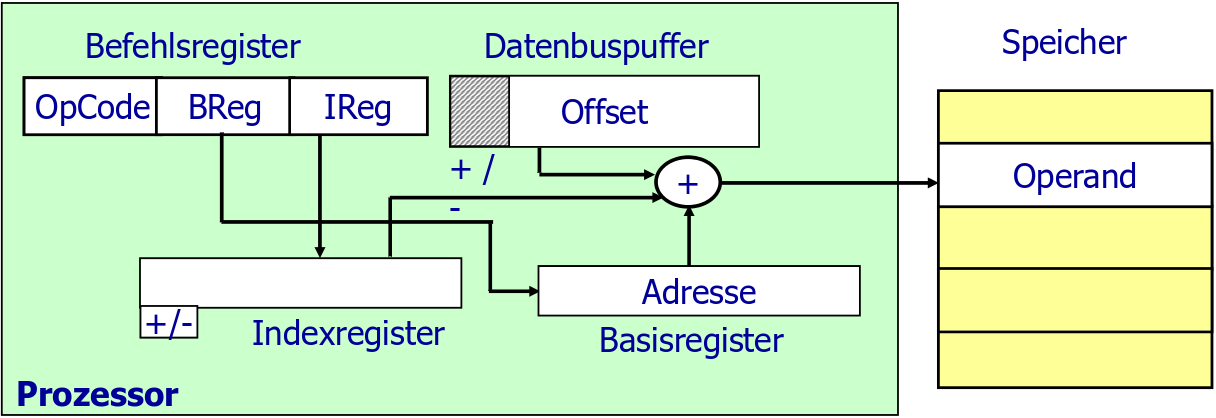
\includegraphics[width=0.33\textwidth]{RegisterRelativeAdressierungMitIndex}
		  \label{RegisterRelativeAdressierungMitIndex}
		\end{figure}
	\end{enumeration}

	\item \underline{Programmzähler-relative Adressierung}: Effektive Adresse = Befehlszählerstand + Offset (im Befehl angegeben) - erlaubt Programme im Hauptspeicher zu verschieben \\* \textbf{Beispiel}: \code{LBRA \$7FFF} (verzweige \emph{unbedingt} zu Speicherzelle, deren Adressdistanz zu Programmzähler \code{\$7FFF} ist)
\end{items}